%\section{Distribution of IVOA Virtual Observatories Worlwide and its Projects}
\section{IVOA Virtual Observatories Worldwide}

Astronomy has always been a data-driven science, and as such, 
the digital revolution have completely change the astronomical practice.
In fact, the actual presence of the astronomer on site is every
day less required for performing observations, and data sharing, reduction
and collaboration is easier than ever. 

However, the paradigm change 
does not stop here, because astronomers have to front the main challenge of
21st century science: data deluge. It is a fact that astronomical data will
strongly increase both in size and in quantity on the next decade due to various
reasons, including the building of large projects like ALMA and E-ELT, 
the improvement or deployment of new instruments, and the execution of 
large astronomical surveys like the LSST project.
The effort needed to process all this data it will be enormous both
scientifically and in terms of computational capacity. 
In fact, simple search and access procedures become difficult
when too many files are available.

Consequently, is desirable to distribute the scientific and the computational 
load in several centers, each one specialized on certain data and instruments
to avoid redundancy of observations and work. However, this distributed work
should be organized to be able to interoperate between centers.
In this context, 0rganizing the inherent diversity of several countries working together, 
with different goals, working-style and budgets is the central objective of
the IVOA.


\subsection{The IVOA}
\rem{MA}{Check this section}

Since June 2002, virtual observatory projects have come to integrate the
International Virtual Observatory Alliance (IVOA) under the \textbf{Guidelines
for Participation\footnote{\url{http://www.ivoa.net/documents/latest/IVOAParticipation.html}}}. 
These projects are funded through national/international governmental and private programs in
collaboration with various centers of scientific studies, universities and
others. Who integrate this project, the Virtual Observatory (VO), share
knowledge between them and the community in a standardized manner. They
themselves are who develop these standards for data exchange and
interoperability. 

The table \ref{table:partners} shows the partners of IVOA to
November 2013.\\

\begin{table*}[h!t]
	\centering
	\begin{tabular}{|l|p{9cm}|l|}
	\hline
	\textbf{Project} & \textbf{Organizations} & \textbf{URL} \\
	\hline
	NOVA (Argentina) & 8 institutions, National Universitiy of La Plata, Faculty of Astronomical Sciences and Geophysics of la Plata & \url{http://nova.conicet.gov.ar/} \\
	\hline
	ARVO (Armenia) & Digital First Byurakan Survey, DFBS & \url{http://www.aras.am/Arvo/arvo.htm} \\
	\hline
	AstroGrid (United Kingdom) & Particle Physics and Astronomy and Research Council (PPARC) Sciency \& Technology Facilities Council (STFC) &\url{http://www.astrogrid.org/} \\
	\hline
	Aus-VO (Australia) & Linkage Infrastructure, Equipment and Facilities & \url{http://aus-vo.org.au/} \\
	\hline
	BRAVO (Brazil) & Brazilian Astronomical Society, SBA National Institue for Science and Technology in Astrophysics, INCT-A & \url{http://www.lna.br/bravo/} \\
	\hline
   	CVO (Canada) & Canadian Astronomy Data Centre & \url{http://www.cadc-ccda.hia-iha.nrc-cnrc.gc.ca} \\
	\hline
    ChiVO (Chile) & 5 universities, supported by ALMA, REUNA & \url{http://www.chivo.cl/} \\
	\hline
    China-VO (China) & National Astronomical Observatories. Chinese Academy of Sciences & \url{http://www.china-vo.org/} \\
%	\hline
%    ESA-VO &
%    \url{http://www.sciops.esa.int/} \\
	\hline
	EURO-VO (Europe) & Continuation of Astrophysical Virtual Observatory, European Commision and six organization & \url{http://www.euro-vo.org/} \\
	\hline
	GAVO (German) & Federal Ministry of Education and Research (BMBF) & \url{http://www.g-vo.org/} \\
	\hline
	HVO (Hungary) & & \url{http://hvo.elte.hu/en/} \\
	\hline
	VObs.it (Italy) & Italian National Institute for Astrophysics, Information System Units & \url{http://vobs.astro.it/} \\
	\hline
	JVO (Japan) & National Astronomical Observatory of Japan, Fujitsu & \url{http://jvo.nao.ac.jp/}\\
	\hline
	VO-France (France) & & \url{http://www.france-vo.org/} \\
	\hline
	RVO (Russia) & & \url{http://www.inasan.rssi.ru/eng/rvo/} \\
	\hline
	SVO (Spain) & Centro de Astrobiología (INTA-CSIC). Artificial Intelligence Department of the National University of Distance Education. University of Cádiz and Center of Scientific and Academic Services of Catalonia (CESCA) & \url{http://svo.cab.inta-csic.es/} \\
	\hline
	SA$^3$ (South Africa) & National Research Fundation. South African Astronomical Observatory. Hartebeesthoek Radio Astronomy Observatory. Square Kilometer Array South Africa & \url{http://www.sa3.ac.za/} \\
	\hline
	UkrVO (Ukrania) & \url{http://www.ukr-vo.org/} \\
	\hline
	VAO (United States) & National Science Foundation, NSF. National Aeronautics and Space Administration, NASA. Associated Universities, Inc, AUI. Association of Universities for Reseach in Astronomy, AURA & \url{http://www.usvao.org/} \\
	\hline
	VOI (India) & Inter University Center for Astronomy and Astrophysics. Ministry of Communication and Information Technology & \url{http://vo.iucaa.ernet.in/~voi/} \\
	\hline
	\end{tabular}
	\caption{IVOA Partners}
	\label{table:partners}
\end{table*}

Almost half of IVOA virtual observatories are supported in Europe\footnote{The
Observatoire Virtuel France is ommited in \textbf{Europe} subsection of
\textbf{List of Virtual Observatories} section by lack of the information.} 9 of
the total; 1 belong to Africa, 1 to Australia, 2 to North America, 3 to South
America and 5 to Asia. Figure~\ref{} shows the pretense of the IVOA's membership
worldwide.\\

\rem{MA}{A little propaganda of the last member :P}

%\begin{figure}%[h]
%\begin{center}
%	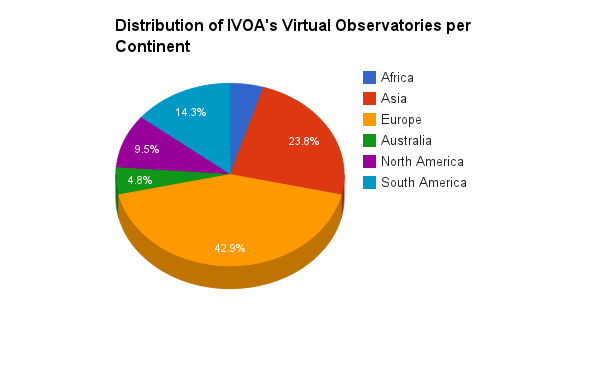
\includegraphics[scale=0.6]{img/vo_distribution.png}
%	\caption{International Virtual Observatory Alliance distribution per
%             continent.}
%\end{center}
%\end{figure}

\begin{figure}%[h]
\begin{center}
	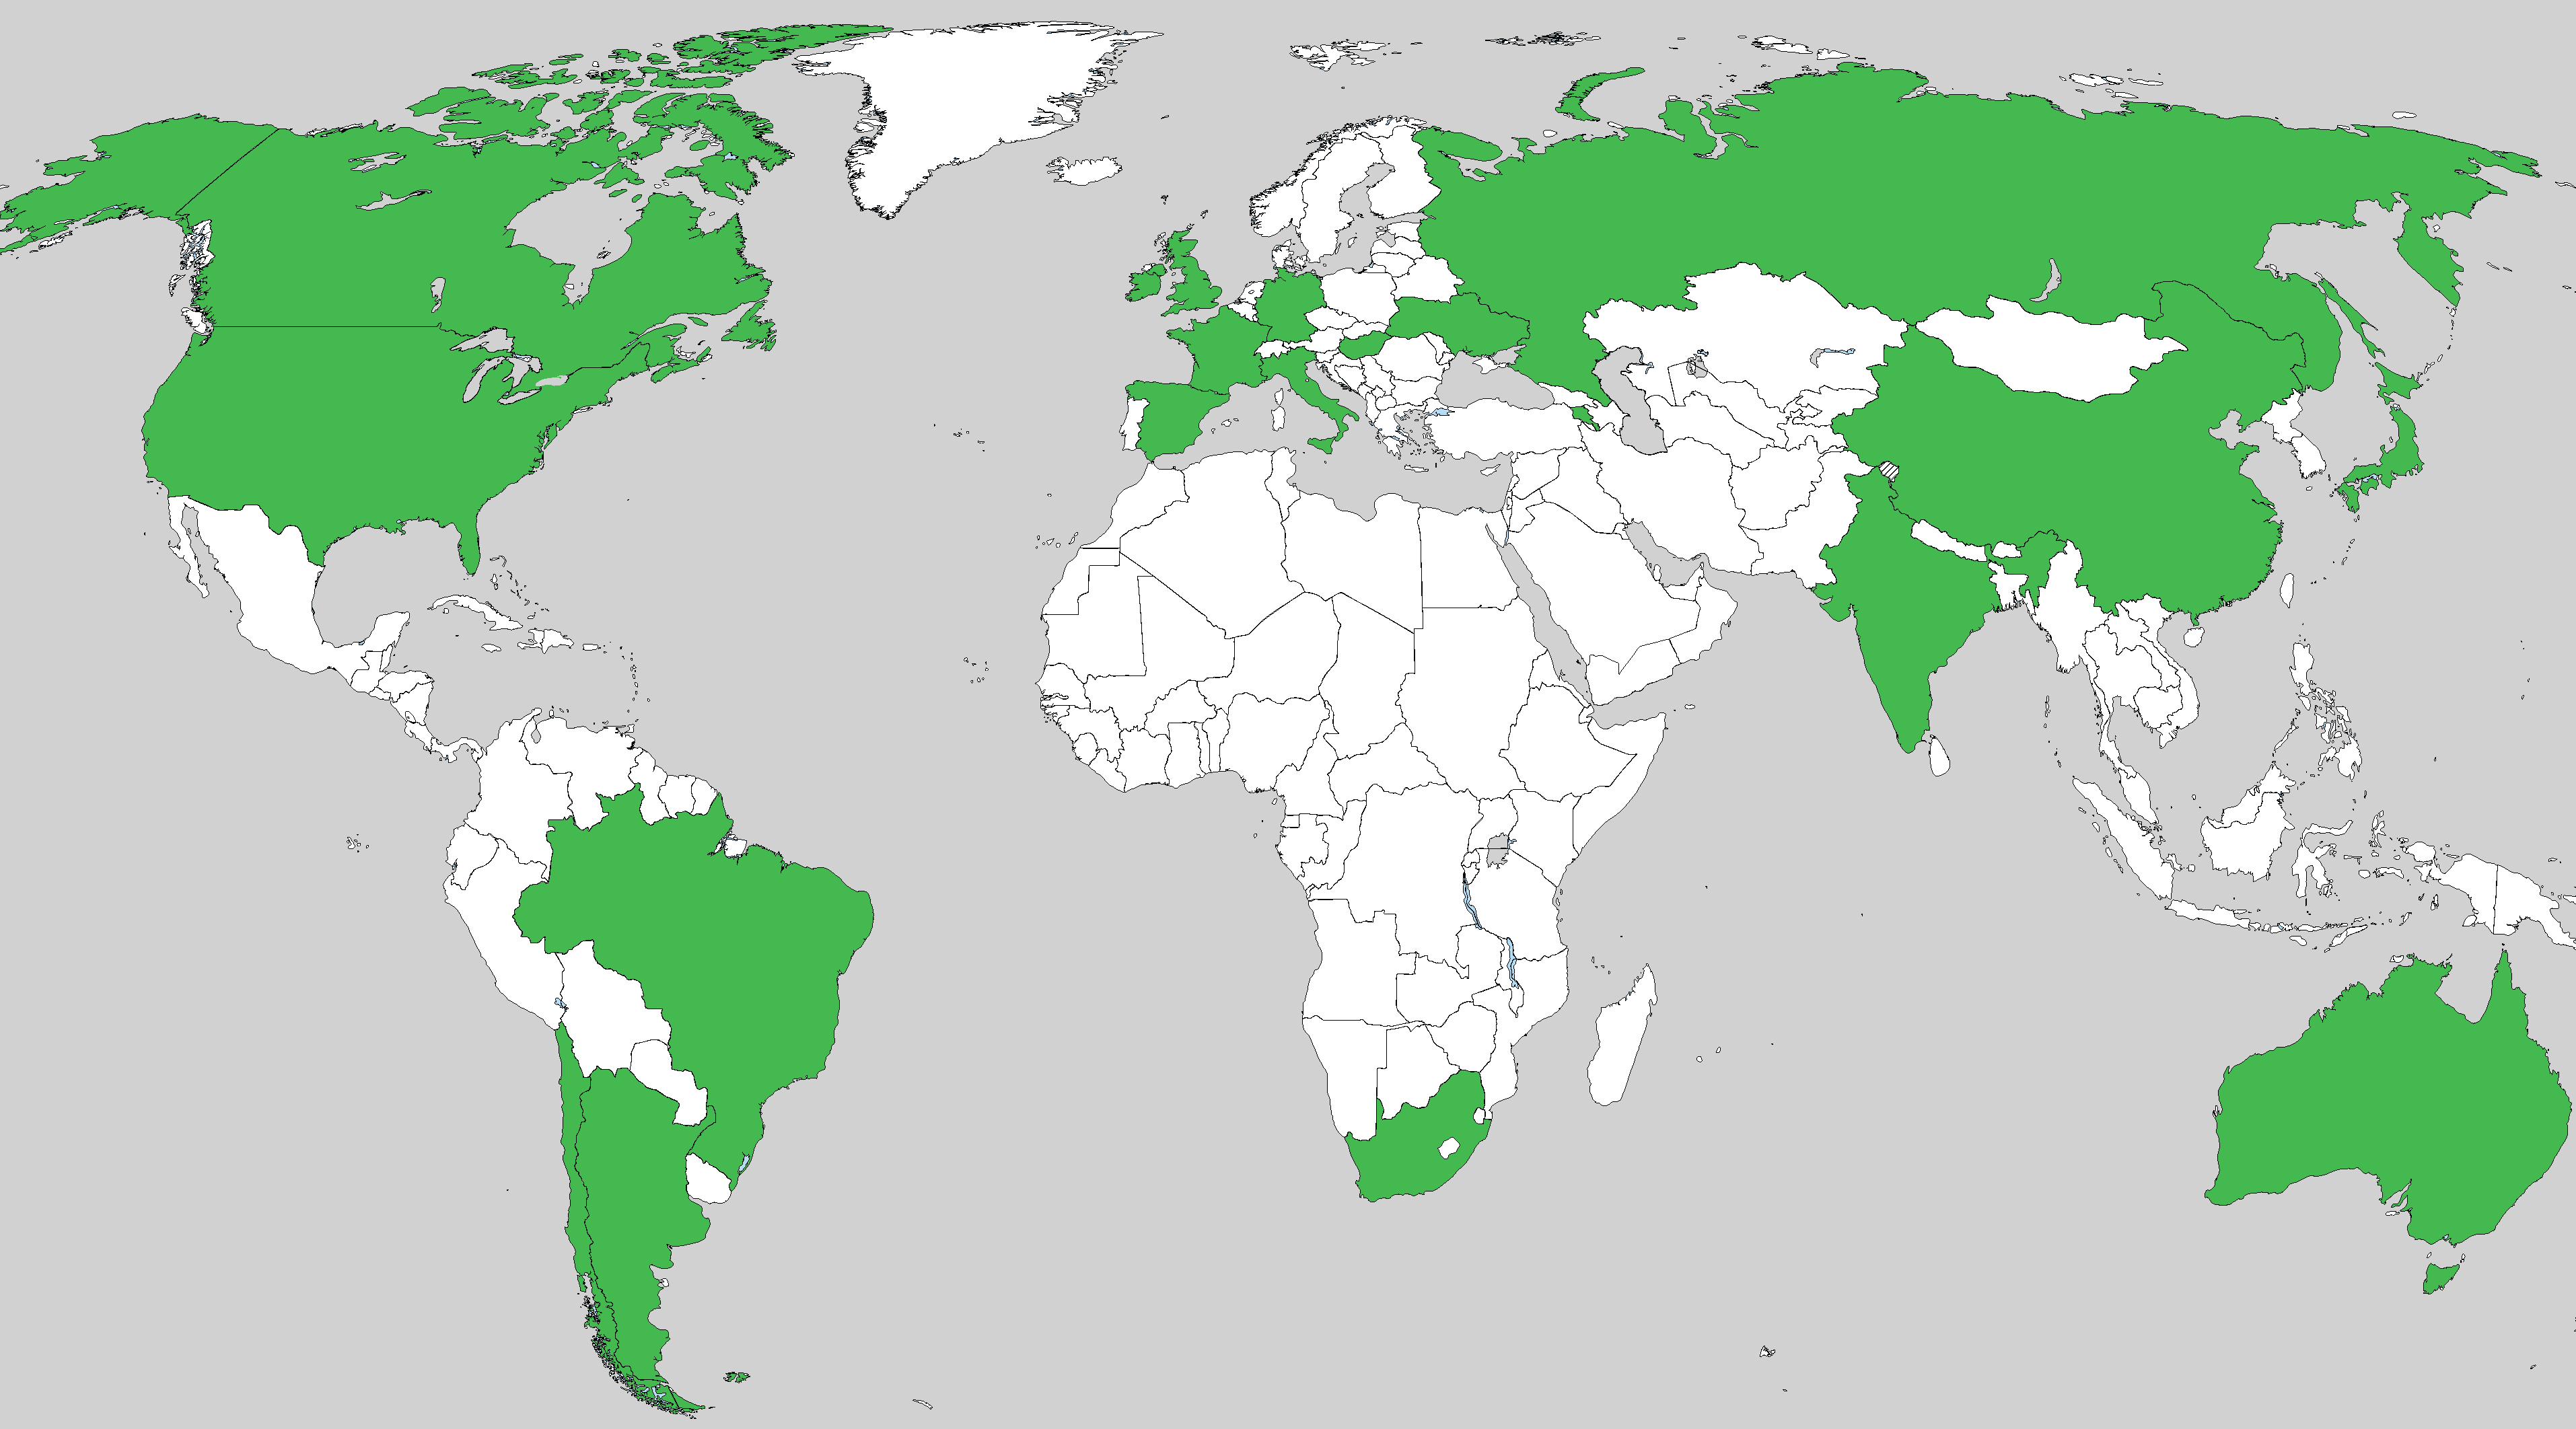
\includegraphics[width=0.9\linewidth]{img/VO-worldwide.png}
	\caption{International Virtual Observatory Alliance presence in the world.}
\end{center}
\end{figure}

\rem{JA}{A lot of initiatives converges in one and only VO. Access worldwide to 
scientists.}

\rem{MA}{subsec: Put here the infrastructure and the organizations}
%\subsection{Infrastructure}
%\begin{itemize}
%\item \textbf{EURO-VO}
%\item \textbf{EURO-VO Data Centre Alliance (EuroVO-DCA)}:
%it is supported by the European Union (EU) in the framework of the FP6
%e-Insfraestructure Communication Network Development initiative (project
%RI031675). It began on 1st of September, 2006, and ended on 31th of December,
%2008.
%\item \textbf{EURO-VO Astronomical Infraestructure for Data Access
%              (EuroVO-AIDA)}:
%it is supported by the European Union (UE) in the framework of the FP7
%e-Infrastructure Scientific Research Repositories initiative (project
%RI2121104). It began on 1st of February, 2008, and ended on 31th of July, 2010.
%\end{itemize}

%\subsection{Organizations}
%\rem{MA}{Funding and Support: important actors of a VO}
%\begin{itemize}
%	\item \textbf{CVO}
%	\item Canadian Astronomy Data Centre
%	\item \textbf{VAO}
%	\item National Science Foundation, NSF
%	\item National Aeronautics and Space Administration, NASA 
%	\item Associated Universities, Inc, AUI.
%	\item Association of Universities for Reseach in Astronomy, AURA
%	\item \textbf{BRAVO}
%	\item Brazilian Astronomical Society, SBA
%	\item National Institue for Science and Technology in Astrophysics, INCT-A
%	\item \textbf{ChiVO}
%	\item 5 universities, supported by ALMA, REUNA
%	\item \textbf{NOVA}
%	\item 8 institutions, National Universitiy of La Plata, Faculty of Astronomical 
%		Sciences and Geophysics of la Plata
%	\item \textbf{ArVO}
%	\item Digital First Byurakan Survey, DFBS
%	\item \textbf{AstroGrid}
%	\item Particle Physics and Astronomy and Research Council  (PPARC)
%	\item Sciency \& Technology Facilities Council (STFC)
%	\item \textbf{ESA-VO}
%	\item Study
%	\item \textbf{EURO-VO}
%	\item Continuation of Astrophysical Virtual Observatory, European Commision and six organization
%	\item \textbf{GAVO}
%	\item Federal Ministry of Education and Research (BMBF)
%	\item \textbf{SVO}
%	\item Centro de Astrobiología (INTA-CSIC)
%	\item Artificial Intelligence Department of the National University of Distance Education
%	\item University of Cádiz and Center of Scientific and Academic Services of Catalonia (CESCA)
%	\item \textbf{VObs.it}
%	\item Italian National Institute for Astrophysics
%	\item Information System Units
%	\item \textbf{Ukrainian}
%	\item Ukrainian Astronomical Association (UAA)
%	\item \textbf{SA$^3$}
%	\item National Research Fundation
%	\item South African Astronomical Observatory
%	\item Hartebeesthoek Radio Astronomy Observatory
%	\item Square Kilometer Array South Africa 
%	\item \textbf{China-VO}
%	\item National Astronomical Observatories
%	\item Chinese Academy of Sciences
%	\item \textbf{JVO}
%	\item National Astronomical Observatory of Japan
%	\item Fujitsu
%	\item \textbf{VOI}
%	\item Inter University Center for Astronomy and Astrophysics
%	\item Ministry of Communication and Information Technology
%	\item \textbf{Aus-VO}
%	\item Linkage Infrastructure, Equipment and Facilities
%\end{itemize}



%\rem{MA}{subsec: Development lines of VOs and data speciality}

% If Chile became part of International Virtual Observatory Alliance, the
% distribution of IVOA's members per continent will be as shown in the figure
% 2. \\

%\begin{comment}
%\begin{figure}%[h]
%\begin{center}
%	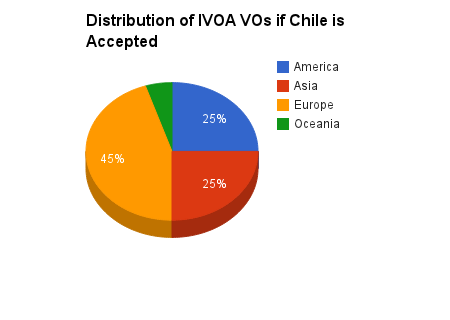
\includegraphics[width=110mm]{img/if_chile.png}
%	\caption{International Virtual Observatory Alliance distribution per
%             continent if Chile is accepted.}
%\end{center}
%\end{figure}
%\end{comment}

%Without considering the status of the internal projects of the virtual
%observatories, the membership of Chile would contribute to the cooperation,
%development and interoperability from America in the same percent that Asia.
%Furthermore, this fact would be very significant, because a large numbers of
%astronomical centers like observatories are placed in this country.  For now, is
%intended to work with a certain quantity of data of ALMA.\\
